%%%%%%%%%%%%%%%%%%%%%%%%%%%%%%%%%%%%%%%%%%%%%%%%%%%%%%
%
%     Oil Sands Paper 
%	Version Matching Word Document V25
%     
%
%%%%%%%%%%%%%%%%%%%%%%%%%%%%%%%%%%%%%%%%%%%%%%%%%%%%%%

\title{ {\bf A Symbiotic System Model for the Development of Canadian Oil Sands  } \\ \vspace{11pt} \small{
 And The Potential For Positive Impact On The Decision To Build The Keystone Pipeline} }

\author{
AUTHORS
}

\date{}

\documentclass[11pt]{article}

\usepackage{amsmath}
\usepackage{amssymb}
\usepackage{amsthm}
\usepackage{color}
\usepackage{graphicx}
\usepackage{enumerate}
\usepackage{colortbl}
\usepackage[table]{xcolor}
\setlength{\textwidth}{6.5in}
\setlength{\textheight}{9.2in}
\setlength{\voffset}{-1.1in}
\setlength{\hoffset}{-0.7in}
\newcommand{\h}[1]{\colorbox{yellow}{#1}}

\begin{document}
\maketitle


%%%%%%%%%%%%%%%%%%%%%%%%%%%%%%%%%%%%%%%%%%%%%%%%%%%%%%
%  Abstract Section
%%%%%%%%%%%%%%%%%%%%%%%%%%%%%%%%%%%%%%%%%%%%%%%%%%%%%%

\begin{abstract}
We propose a symbiotic system model for the development of Canadian Oil Sands: for example, if 10\% of Canadian Oil Sands income (priced at US\$75 per barrel of oil) were to be invested in renewable-energy machines as part of reclamation efforts for the land that is mined, then three significant results can follow. First, we estimate that in 36 years as much CO$_2$ will have been kept from the air from burning coal to make electricity as was released into the air from mining the oil sands and consuming the oil. Second, the investment is a better and more productive alternative to a ``Carbon Tax'' because the money is put directly to use to benefit oil sands development in the short term and renewable power generation in the long term, and the resources remain on the development companies’ balance sheets. Finally, during periods of peak electrical power generation, the power can be sold back to the grid, power electric underground heaters for liquefying bitumen for extraction without mining operations, or to power operations for cleaning contaminated water of Poly-Aromatic Hydrocarbons (PAH), which can be hydrocracked into useful compounds.
\end{abstract}

%%%%%%%%%%%%%%%%%%%%%%%%%%%%%%%%%%%%%%%%%%%%%%%%%%%%%%
%  1) Introduction Section
%%%%%%%%%%%%%%%%%%%%%%%%%%%%%%%%%%%%%%%%%%%%%%%%%%%%%%

\section{Introduction}

\subsection{Motivation}

The Northern Alberta region contains 98\% of the Canadian oil sands and they are divided into three regions:
\begin{itemize}
\item The Athabasca-Wabiskaw deposits region
\item The Cold Lake deposits regions 
\item The Peace River deposits region
\end{itemize}

\indent Together, they cover about 140,200 square kilometers [1]. It is also estimated that these regions hold proven reserves up to 1.75 trillion barrels of bitumen [2]. In addition, 173 billon barrels (10\%) are estimated to be recoverable at current prices using existing mining technology. About two tonnes of oil sands must be dug up, moved, and processed to produce 1 barrel of synthetic oil [3].  \\
\indent Detractors hypothesize that mining, processing, and using the oil from the oil sands will greatly exacerbate global CO$_2$ problems, and extend this argument as a reason for the US to deny permission to grant approval for the Keystone XL pipeline. Proponents say that global CO$_2$ impact will be no different than from other sources of oil, and the pipeline is safer than rail shipments. 

\subsection{Problem Observation}

The Province of Alberta is currently operating a modest at best energy return per area invested: oil sands are being mined over a vast area which destroy large swaths of forests releasing even more carbon into the atmosphere while also generating large lagoons of heavily polluted water. In the spirit of increasing the Energy Return on Investment (EROI) from this vast resource, we present a possible better EROI for the area and the country.  \\

\noindent {\bf Hypothesis:} \\

\emph{The effect of oil sands utilization on climate change does not have to be negative if, as part of land reclamation of the mined oil sands area, developers of the oil sands resource planned and invested for when the oil sands are depleted. One scenario could include for every square kilometer of land to be reclaimed, a 5 MW wind turbine is installed. The power from the turbine can be used for oil sands production, and excess power can also be sold to the grid or be used to clean contaminated. Another possible scenario could include significant coverage of the land to be reclaimed by PV solar panels. } \\
  
\subsection{Method}
We propose a hypothetical economic model which implements renewable energy systems deployed in reclamation lands which offsets CO$_2$ in the long-term. In this model, we calculate the CO$_2$ offset percentage by finding ratio between the amount of Cumulative Ratio Carbon Saved and the amount of Carbon Burned. The Cumulative Ratio Carbon Saved changes according a set of parameters:

\begin{itemize}
\item The choice of renewable system to offset the CO$_2$: wind energy system or solar energy system
\item Deployment of the systems to be located in a percentage area of the oil sands region to be reclaimed
\item Peak Power for a wind turbine or a solar panel
\item The cost per watt (\$/Watt) of the renewable system with the installation included
\item The Reinvestment Policy amount to be either \$0.05/kWh or \$0.07/kWh per year into purchasing more equipment for the deployed energy system 
\item The approximate decommission rate of a wind turbine or solar panel 
\item Different amounts of yearly investments in the renewable energy system based on: 
\begin{itemize}
\item {\bf Case 1:} A portion of the oil sands income (a percentage of a barrel of oil) to be invested in the model instead implementing a Carbon Tax (described in Section 3.1 of this paper)
\item {\bf Case 2:} A portion of the Carbon Tax as a Carbon Reinvestment Tax (described in Section 3.2 of this paper)
\end{itemize}
\end{itemize}

%%%%%%%%%%%%%%%%%%%%%%%%%%%%%%%%%%%%%%%%%%%%%%%%%%%%%%
% 2)  Results Section
%%%%%%%%%%%%%%%%%%%%%%%%%%%%%%%%%%%%%%%%%%%%%%%%%%%%%%

\section{Results}

\subsection{CO$_2$ Offset by Investing in Wind Energy}

Our first economic model is the study of CO$_2$ offset by investing in wind energy only. The initial reinvestment and reclamation hypothesis appears promising, and Figures 1 and 2 show different scenarios for different percentage of investments for US\$75/bbl that will need to be considered by a more detailed investigation.  Table 1 shows the modeling assumptions and the amount of CO$_2$ saved by wind turbines 

\begin{center}
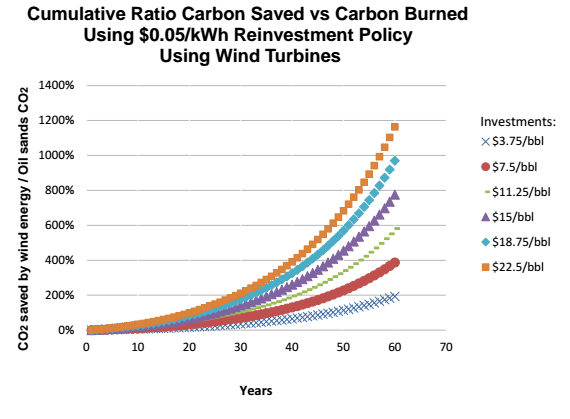
\includegraphics[scale=0.65]{g1.png}
\end{center}
{\bf Figure 1.} Amounts of CO$_2$ offset with different investments in wind energy systems, assuming a wind turbine life expectancy of 20 years, one wind turbine per square kilometer of reclaimed land up to a total of 70,100 square kilometers (50\% of oil sands region), \$2/Watt cost including installation of the wind turbine, and a \$0.05/kWh Reinvestment Policy into purchasing more wind turbines every year.

\begin{center}
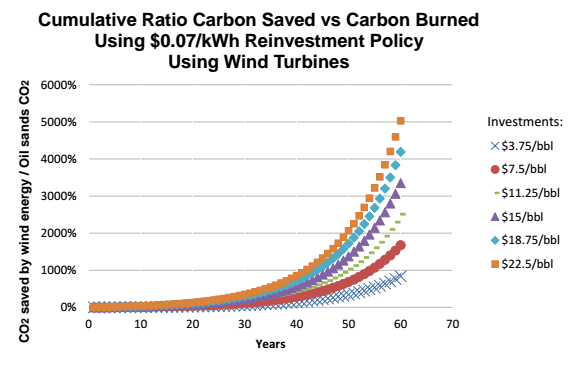
\includegraphics[scale=0.65]{g2.png}
\end{center}
{\bf Figure 2.}  Amounts of CO$_2$ offset with different investments in wind energy systems, assuming a wind turbine life expectancy of 20 years, one wind turbine per square kilometer of reclaimed land up to a total of 70,100 square kilometers (50\% of oil sands region), \$2/Watt cost including installation of the wind turbine, and a \$0.07/kWh Reinvestment Policy into purchasing more wind turbines every year.

\begin{center}
{\bf Wind Energy System Model Specifications}

\begin{tabular}{|l|l|}
\hline
\cellcolor{gray!35} {\bf Description} & \cellcolor{gray!35} {\bf Value} \\
\hline
Turbine Peak Power (MW) & 5 \\
\hline
Capacity factor & 40\% \\
\hline
Land area per turbine (km$^2$) & 1 \\
\hline
Percent land area for wind turbines & 50 \% \\
\hline
area of wind farm (km$^2$) & 70,100 \\
\hline
\hspace{18em} Square miles & 27,383 \\
\hline
\hspace{12em} Square size (miles x miles) & 165 \\
\hline
Number of turbines to be built for land area & 70,100 \\
\hline
Average Power generated (GW) & 198 \\
\hline
Average annual energy produced (TWHr) & 1,734 \\
\hline 
{\bf CO$_2$ saved by wind turbines (Megatonnes/Year)} & {\bf 1,684} \\
\hline
\end{tabular}
\end{center}
\begin{center}
{\bf Table 1.} Modelling assumptions for determining amount of CO$_2$ saved by Wind Turbines
\end{center}

\noindent Other model considerations include:
\begin{itemize}
\item {\bf Wind Turbine Peak Power}
\begin{itemize}
\item The choice of 5 MW/km$^2$ is conservative as forthcoming are 7 MW turbines, although they will require larger spacing.  Even 10 MW turbines are under consideration for production.
%\newpage
\end{itemize}
\item {\bf Wind Turbine Capacity Factor}
\begin{itemize}
\item NREL's median capacity factor to be 40\% for onshore wind turbines
\item With higher hub heights, up to 140m, wind turbine net capacity factor could rise to 50\% (70,100 km$^2$).
\end{itemize}
\item {\bf Land area per turbine}
\begin{itemize}
\item Land area assumed to cover 1 km$^2$ per turbine, many wind farms actually place up to two turbines in this area.
\end{itemize}
\item {\bf Percent land area for wind turbines}
\begin{itemize}
\item Assumption to cover 50\% of the total Alberta tar sands area
\end{itemize}
\item {\bf Cost of installation of wind turbines}
\begin{itemize}
\item Estimated to be \$2/W with the installation.
\end{itemize}
\item {\bf Reinvesment Policy}
\begin{itemize}
\item Assumption to reinvest \$0.05/kWh or \$0.07/kWh into wind turbine purchase and maintenance.
\end{itemize}
\end{itemize}

\subsection{CO$_2$ Offset by Investing in Solar Energy}

Our second model is the study of CO$_2$ offset by investing on solar energy systems. A more modest, but still significant results are obtained with 30\% of the land area reclaimed using arrays of PV cells in Table 2.

\begin{center}
{\bf Solar Energy System Model Specifications}
\begin{tabular}{|l|c|}
\hline
\cellcolor{gray!35} {\bf Description} & \cellcolor{gray!35} {\bf Value} \\
\hline
Percent land area assumed covered by PV fields & 15 \% \\ 
\hline
Area of PV farm (km$^2$) & 14,020 \\
\hline
\hspace{24.5em} (Square miles) & 5,477 \\
\hline
\hspace{19em} Square Size (miles x miles) & 74 \\
\hline
Density of coverage on land designated  for PV fields & 30\% \\
\hline
Area of PV cells (m$^2$) &  6,309,000,000 \\ 
\hline
PV Cell efficiency & 15 \% \\
\hline
Average 24/7 solar insolation April (WH/m$^2$/day) &  \\
\hline
\hspace{29.5em}June & 6,250 \\
\hline
\hspace{28em}January & 1,389 \\
\hline
Average power (assumes 24/7 operation with storage technology) (GW) & \\
\hline
\hspace{29.5em}June & 164 \\
\hline
\hspace{28em}January & 37 \\
\hline
\hspace{28em}Average & 100.405 \\
\hline  
{\bf Total CO$_2$ saved by PV cells (Megatonnes/Year)} & {\bf 854} \\
\hline
\end{tabular}
\end{center}

\begin{center}
{\bf Table 2.} Amount of CO$_2$ saved by not burning coal to produce energy by PV solar panels
\end{center}

Similarly, the behavior of these results are controlled by the amount investment (\$US/bbl), the life expectancy of the solar cells, the peak power of the solar cells, and the (\$/kWh) Reinvestment Policy into purchasing more solar cells. 

%%%%%%%%%%%%%%%%%%%%%%%%%%%%%%%%%%%%%%%%%%%%%%%%%%%%%%
%  3) Discussion
%%%%%%%%%%%%%%%%%%%%%%%%%%%%%%%%%%%%%%%%%%%%%%%%%%%%%%

\section{Discussion}

\subsection{Economic Models}

We hypothesize that a better EROI would be obtained by investing in renewable energy systems emplaced on land to be reclaimed from mining activities. Figure 1 shows an example of the cumulative effect on CO$_2$ emissions over the years with this land reclamation plan, where 50\% of the total oil sands land area being reclaimed include wind turbine installations, one wind turbine per square kilometer, funded by oil revenues and a \$0.05/kWh reinvestment from the wind power generated. Table 3 shows the years to achieve 100\% cumulative CO$_2$ offset by various investment percentage strategies

\begin{center}
{\bf Approximate CO$_2$ Offset Timelines Using the Wind Energy System Model}
\begin{tabular}{|c|c|c|}
\hline
\cellcolor{gray!35} \parbox[t]{5cm} {{ \begin{center} \bf Investment Amount \\  (\$US/bbl) \end{center}}} & \cellcolor{gray!35} \parbox[t]{5cm}{{\bf  \begin{center} Estimated Time with \\ \$0.05/kWh Reinvestment \\ (Years) \end{center} }} & \cellcolor{gray!35} \parbox[t]{5cm}{{\bf \begin{center} Estimated Time with \\ \$0.07/kWh Reinvestment \\ (Years) \end{center}}} \\
\hline
3.75 & 48 & 36  \\
\hline
{\bf 7.5} & {\bf 36} & {\bf 29} \\
\hline
11.25 & 30 & 25 \\
\hline
15 & 26 & 22 \\
\hline
18.75 & 23 & 20 \\
\hline
22.5 & 20 & 18 \\
\hline
\end{tabular}
\end{center}

\begin{center}
{\bf Table 3.} Estimated timeline for 100\% CO$_2$ offset for wind energy systems based on specific investment amounts (\$US/bbl) and a \$0.05/kWh or \$0.07/kWh Reinvestment Policy into buying more wind turbines.
\end{center}

\indent These scenarios are dependent on four parameters: the percentage of investment per barrel of oil sand (\$US/bbl), the life expectancy of wind turbines, the cost per watt (\$/Watt), the choice of wind turbine peak power, and the Reinvestment Policy amount for new equipment (\$/kWh). If we invest the same amount each year eventually we hit a steady state for number of turbines vs. carbon emissions. The ability to achieve a 100\% offset is sensitive to the \$/kWh reinvestment from power generated. For example, with 20-year life expectancy and \$0/kWh of reinvestment we need the percentage of investment per barrel to be bigger than \$25/bbl to ultimately reach 100\% ever.
The solar model presented in Section 2.2 would in fact never totally offset the CO$_2$ created by mining and using the oil sands oil. This is due to the decommission period of the solar panels. Current panel technology and effective installation costs prevent being able to offset the CO$_2$ attributed to oil sands. However, a significant amount of CO$_2$ reduction could be accomplished and therefore the analysis of this scenario was presented for completeness.  \\
\indent In the long term, it would be possible to send power generated out along the power lines that recently have been built to provide power to the oil sands region, thus enabling coal-fired power plants in the other regions to be phased out. Furthermore, it is common for the return on investment (ROI) period for a wind turbine to be about 15 years [4], which means the \$7.5/bbl invested is actually fully recouped in 10 years and then onward the wind turbine becomes a net income producer and a profitable source of income for the company operating the wind turbine

\subsection{Carbon Reinvestment Tax}
We can think of the economic models from Figure 1 and Figure 2 from a carbon footprint as a function of a carbon reinvestment tax perspective.

\begin{center}
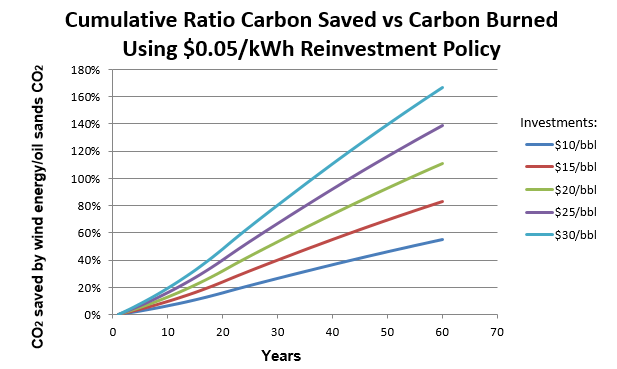
\includegraphics[scale=0.65]{g3.png}
\end{center}
\begin{center}
{\bf Figure 3.}  A Carbon Reinvestment Tax is more affordable in the long term.
\end{center}

We can look at the Carbon Reinvestment Tax as a fraction from the Carbon Tax that companies invest in themselves.

\begin{center}
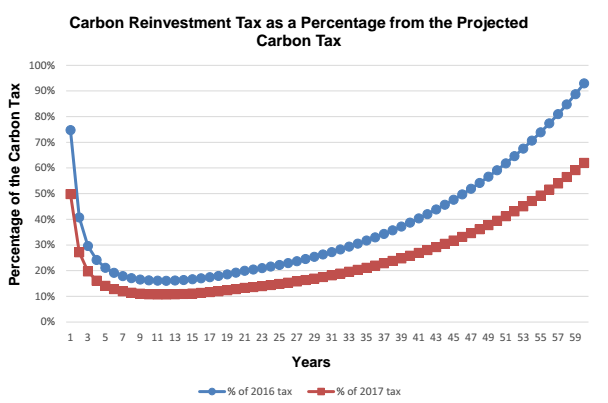
\includegraphics[scale=0.65]{g4.png}
\end{center}
\begin{center}
{\bf Figure 4.} A Carbon Reinvestment Tax as a Percentage of the Carbon Tax
\end{center}

Figure 4 shows how we can take a fraction amount of the proposed Carbon Tax to fund the energy systems. This proportion amount out of a Carbon Tax will increase over time, but proves to be a better solution in the long term. Considering the economic model investment of \$7.5/bbl with a Reinvestment Policy of \$0.05/kWh 

\subsection{Possible Uses of Excess Power Generated}

\indent Companies could benefit from the extra power generated by the wind turbines. It benefits the oil sands companies directly and immediately because they can use the electric power for production of the oil sands instead of having to build more transmission lines, or install small nuclear reactors [5] to bring power in for which they then have to pay to use. \\
\indent In research published in February 2014, the International Council of Clean Transportation and NNFCC, a consultancy, concluded that biofuels made from waste could provide 16\% of Europe’s transport fuels by 2030 [6] and it would create an entirely new industry sector as current production is close to zero. In addition, the International Energy Agency (IEA) calculates that the cost of producing regular gasoline will rise from \$0.54 per litre of gasoline equivalent in 2010 to \$0.82 per litres of gasoline equivalent in 2030. By contrast, the cost of advanced biofuel production will fall from \$1.05-\$1.15 per litre of gasoline equivalent in 2010 to \$0.80-\$1 in 2030 [7]. \\
\indent Other potential applications include selling electricity back to the grid, cleaning contaminated water, exploring the possibility using pumped-storage hydroelectricity, and powering underground electric heaters as an alternative to pumping steam underground for bitumen extraction

\subsection{Mitigations, Transitions, and Adjustments with Labour Unions}
\indent Unions are opposed to building the Keystone XL pipeline not just for environmental reasons, but also for economic reasons as well. The model presented here constitutes a symbiotic approach to mitigate the situation in case the pipeline ever gets built. The mitigation development we present in this paper could be treated, politically, as a way of ``forward planning'' as we would already have a model that could mitigate the situation beforehand. This would save significant time and speed up the negotiation process for the parties involved.  \\
\indent The overall goal of the economic model presented is to contribute to global efforts to slow and limit climate change. Resource industries face a special challenge, and bear a special responsibility.

%%%%%%%%%%%%%%%%%%%%%%%%%%%%%%%%%%%%%%%%%%%%%%%%%%%%%%
%  4) Conclusion Section
%%%%%%%%%%%%%%%%%%%%%%%%%%%%%%%%%%%%%%%%%%%%%%%%%%%%%%

\section{Conclusion}
\indent This paper showed that a symbiotic model to short and long term energy needs can lead to an overall reduction in atmospheric CO$_2$. In Section 3.1, we discussed that we could found our economic model by taking from a percentage of the oil sands income instead of having a Carbon Tax. In Section 3.2, we explored a Carbon Reinvestment Tax as a function of a Carbon Tax and we argued that the reinvestment tax is better suited than a Carbon Tax. \\
\indent It is appears to be economically and politically prudent to undertake as soon as possible a project to install a reasonable number of wind turbines on reclaimed oil sands land in order to better investigate the hypothesis presented here to ascertain true costs, risks, and benefits with respect to ultimately widespread application of this reclamation strategy.

%%%%%%%%%%%%%%%%%%%%%%%%%%%%%%%%%%%%%%%%%%%%%%%%%%%%%%
% Acknowledgments Section
%%%%%%%%%%%%%%%%%%%%%%%%%%%%%%%%%%%%%%%%%%%%%%%%%%%%%%

\section*{Acknowledgments}
\indent The co-authors of this paper would like to deeply thank Professor Alexander H. Slocum for providing the vision behind this project and the idea that shaped the economic models for wind and solar energy presented in this paper. His passion and uncanny love for energy systems to solve humanity’s grand challenges makes him a truly remarkable role model and a great source of inspiration. \\
\indent We would also like to show our gratitude to Canadian labour union Unifor who saw the vision of this project and provided insightful ideas that were key in this paper. Finally, we also thank economist Jim Stanford who gave us comments that greatly improved this paper. 


%%%%%%%%%%%%%%%%%%%%%%%%%%%%%%%%%%%%%%%%%%%%%%%%%%%%%%
%  Bibliography Section
%%%%%%%%%%%%%%%%%%%%%%%%%%%%%%%%%%%%%%%%%%%%%%%%%%%%%%

\begin{thebibliography}{9}
\bibitem{lamport94}
 Alberta Energy. ``About Oil Sands: Facts and Statistics''. Retrieved on March 13, 2014 from Alberta Energy Website: http://www.energy.alberta.ca
 
 \bibitem{lamport94}
  Alberta Environment. (2008). ``Alberta's Oil Sands: Opportunity, Balance''. Retrieved on March 19, 2014 from Alberta Environment Website: http://environment.alberta.ca
 
\bibitem{lamport94}
 Alberta Energy. ``Oil Sands 101''. Retrieved on August 20, 2014 from Alberta Energy Website: http://www.energy.alberta.ca

 \bibitem{lamport94}
 Moloney, C. (2014). ``SmallWind Turbine: What Is the Payback Period''. Retrieved on June 26, 2014 from Poplar Network Website: http://www.poplarnetwork.com
 
 \bibitem{lamport94}
 Daly, J. (2014). ``Canada Considering Nuclear Reactors in Alberta Tar Sands Fields''. Retrieved on April 2, 2014 from Oil Price Website: http://oilprice.com
 
 \bibitem{lamport94}
 UPM Biofuels. (2014). ``Waste-Based Biofuels Sector Needs Smarter EU 2030 Package To Realize Its High Potential''. Retrieved on April 19, 2014 from UPM Biofuels Website: https://www.upmbiofuels.com
 
 \bibitem{lamport94}
 Oliver, C. (2014). ``Biofuels: Wasted energy''. Retrieved on April 17, 2014 from Financial Times Website: http://ft.com	

\end{thebibliography}

\end{document}
